\documentclass[t]{beamer}
\usepackage{amsmath}
\usepackage{movie15}

\usetheme{Warsaw}
%\usecolortheme{lily}
\usefonttheme[onlymath]{serif}

\usepackage[english]{babel}
%\usepackage{palatino}
\usepackage{helvet}
%\usepackage{fourier}
\title{Time Synchronization: Progress Report}
\author{Fasika Assegei}
\date{\today}

\begin{document}

\begin{frame}
\titlepage
\end{frame}
\begin{frame}
\frametitle{Absolute time ...} \centering
 \textbf{\textit{``A man with a watch knows what time it is. A man with two watches is never sure.''}
}
\newline
Segal's Law
\begin{figure}
\centering
\end{figure}
\end{frame}

%\begin{frame}
%    \includemovie[playerid=MACR]{.5\linewidth}{.375\linewidth}{video.mpg}
%\end{frame}

%\section*{Outline}
\frame{\tableofcontents}

\section{Frequency Offset}

\begin{frame}
    \frametitle{Clock Drift}
   \begin{equation}
    \centering
f_i(t) = f_o + \Delta f + f_d(t-t_o) + f_e + f_r(t)
\end{equation}
where\newline
      $f_i$ = phase, or time error \newline
      $f_0$ = nominal frequency of the clock - $32768KHz$ \newline
      $\Delta f$ = calibration error - $30 ppm$ \newline
      $f_d$ = the frequency drift due to aging - $3ppm$ per year \newline
      $f_e$ = frequency variation due to temprature - $-0.035ppm/C^2$ \newline
      $f_r$ = short-term frequency instability due to noise \newline
\end{frame}

\begin{frame}
\frametitle{Frequency variation with Temperature}
 \begin{figure}
  \includegraphics[width=0.6\textwidth]{clock_temp}
  \caption{Frequency variation with temperature}
 \end{figure}
\end{frame}

\begin{frame}
\frametitle{Clock Drift}
\begin{figure}
\centering
<<<<<<< .mine
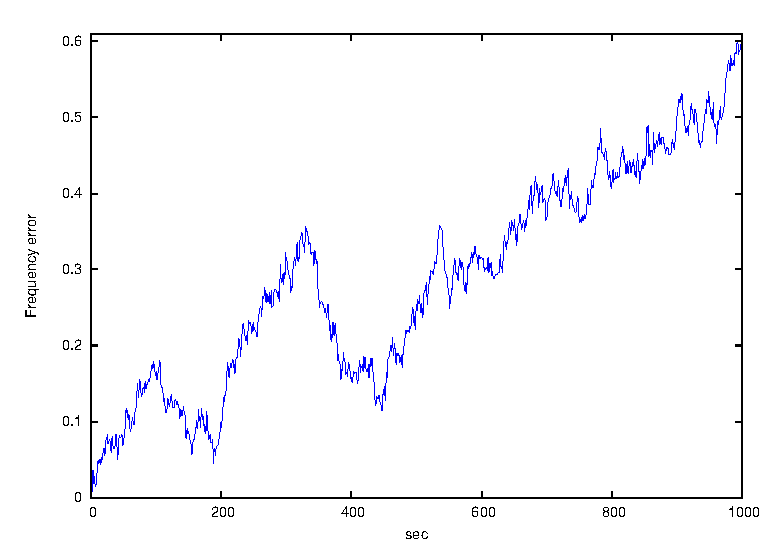
\includegraphics[width= 0.75 \textwidth]{freq_var}
=======
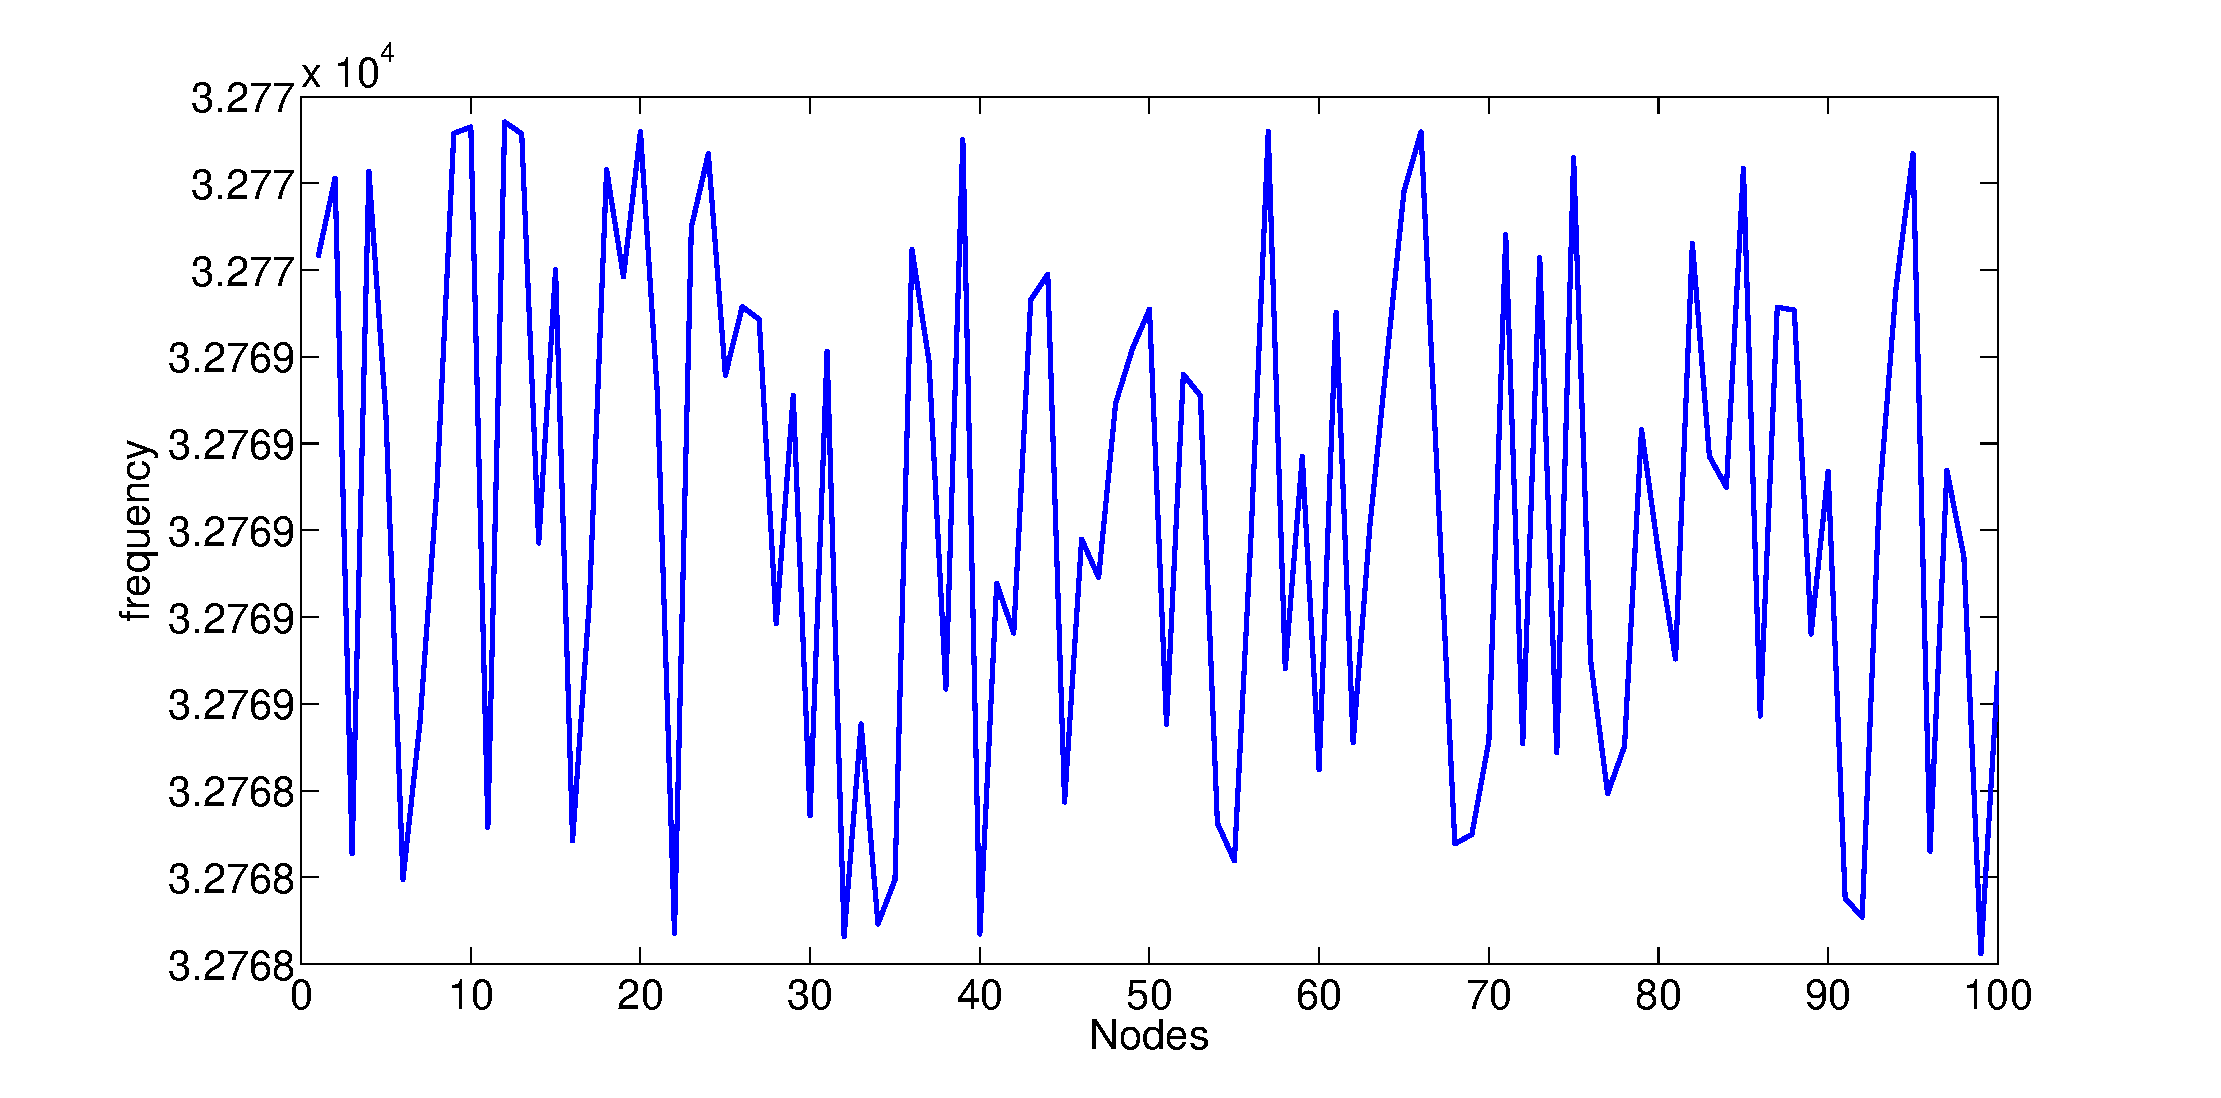
\includegraphics[width= 0.75 \textwidth]{frequency_error}
>>>>>>> .r35
\caption{Frequency variation for different clocks}
\end{figure}
\end{frame}

%\begin{frame}
%\frametitle{Clock Drift effect on Node time}
%\begin{figure}
%\centering 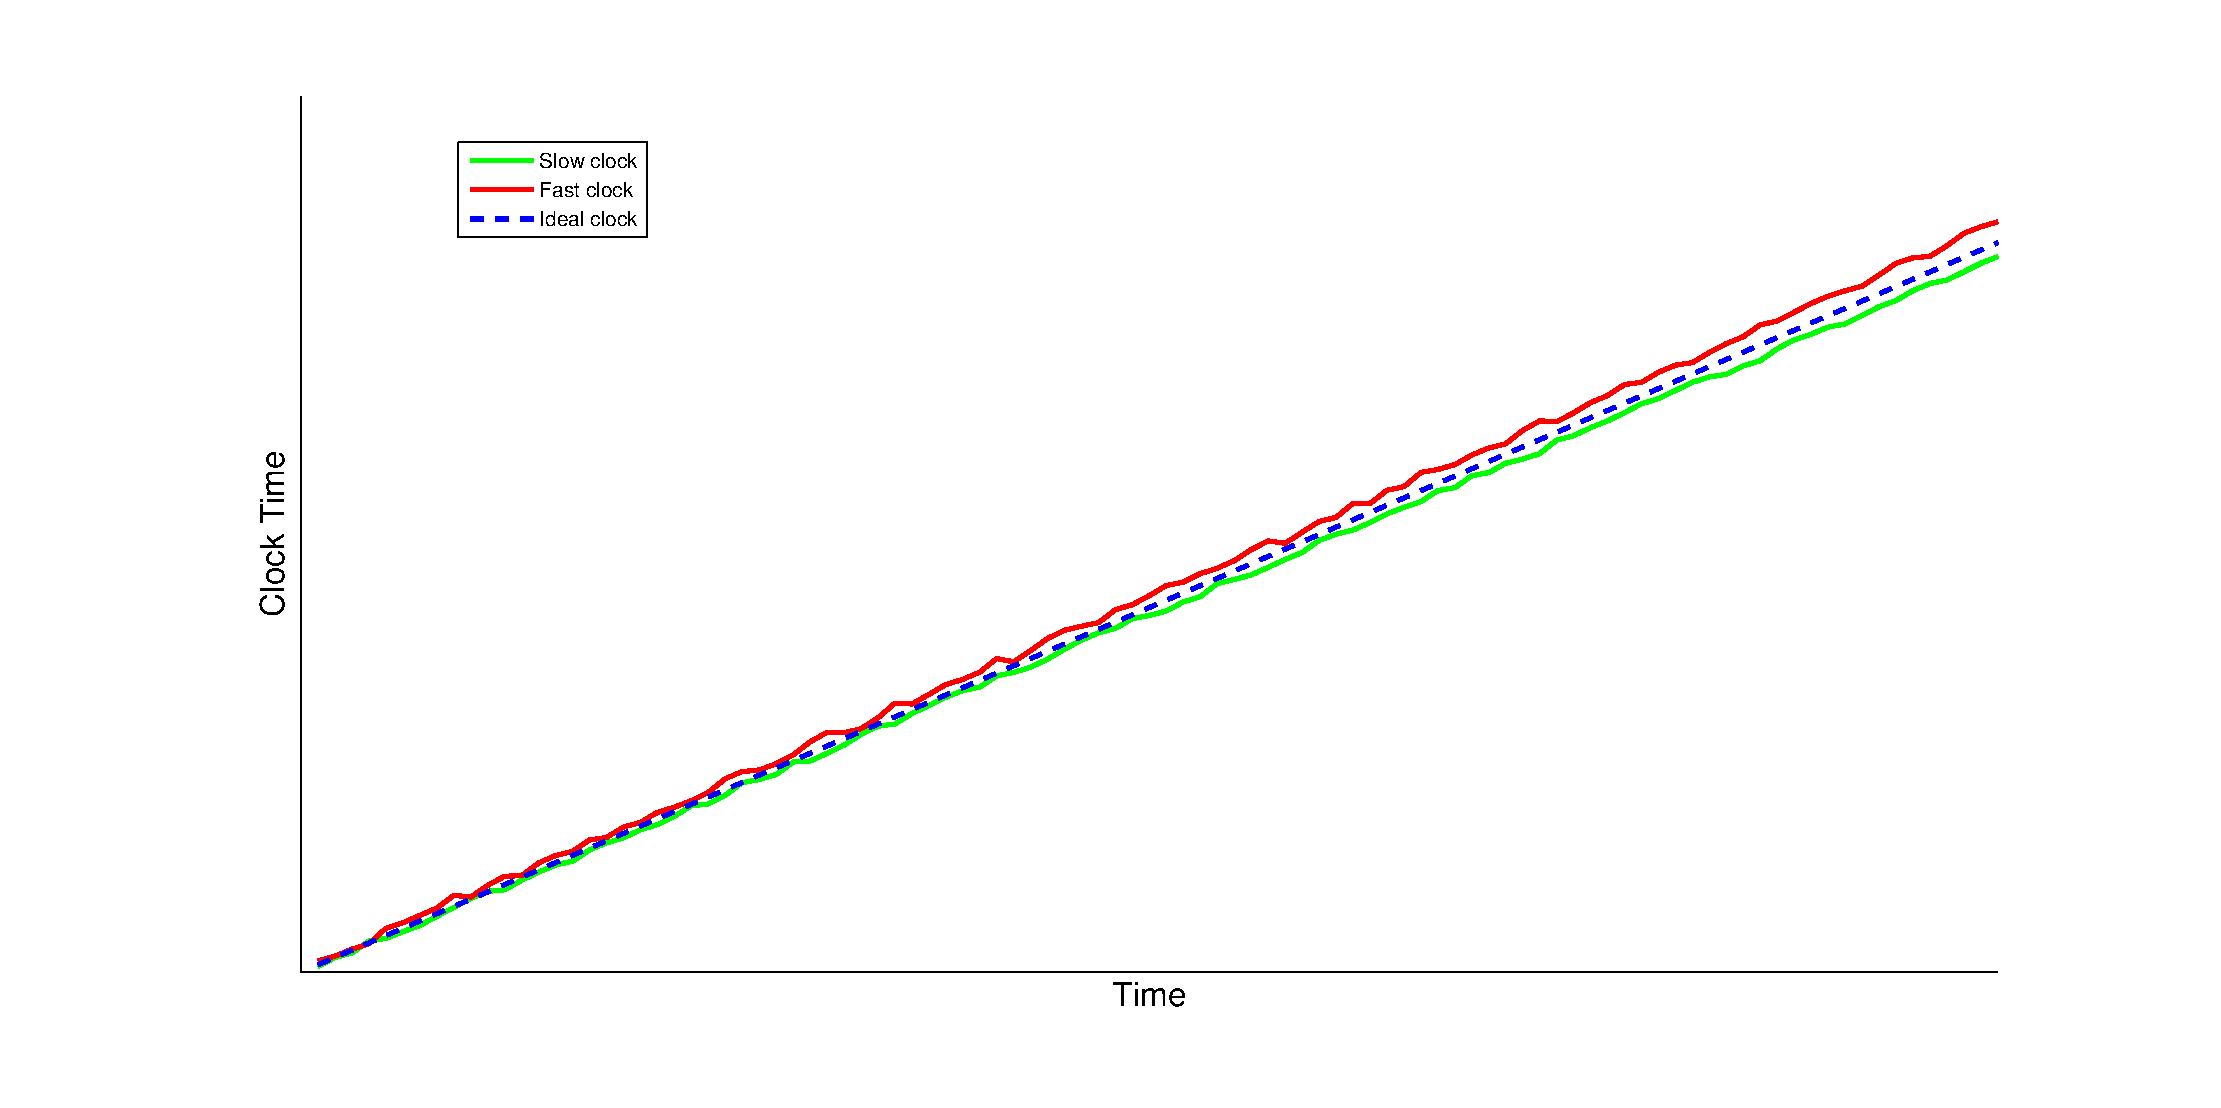
\includegraphics[width= 1\textwidth]{clocktimevsrealtime}
%\caption{Clock time versus real time}
%\label{fig:clocktimevsrealtime}
%\end{figure}
%\end{frame}

\begin{frame}
\frametitle{Worst Case Scenarios}
\begin{equation}
    \centering
f_i(t) = f_o + \Delta f + f_d(t-t_o) + f_e + f_r(t)
\end{equation}
Assuming the maximum deviations ,
\begin{equation}
\Delta f_{max} = 1.0117 Hz
\end{equation}
for a slow clock and
\begin{equation}
 \Delta f_{min} = 0.95436 Hz
\end{equation}
for a fast clock.
\end{frame}

\begin{frame}
\begin{figure}
 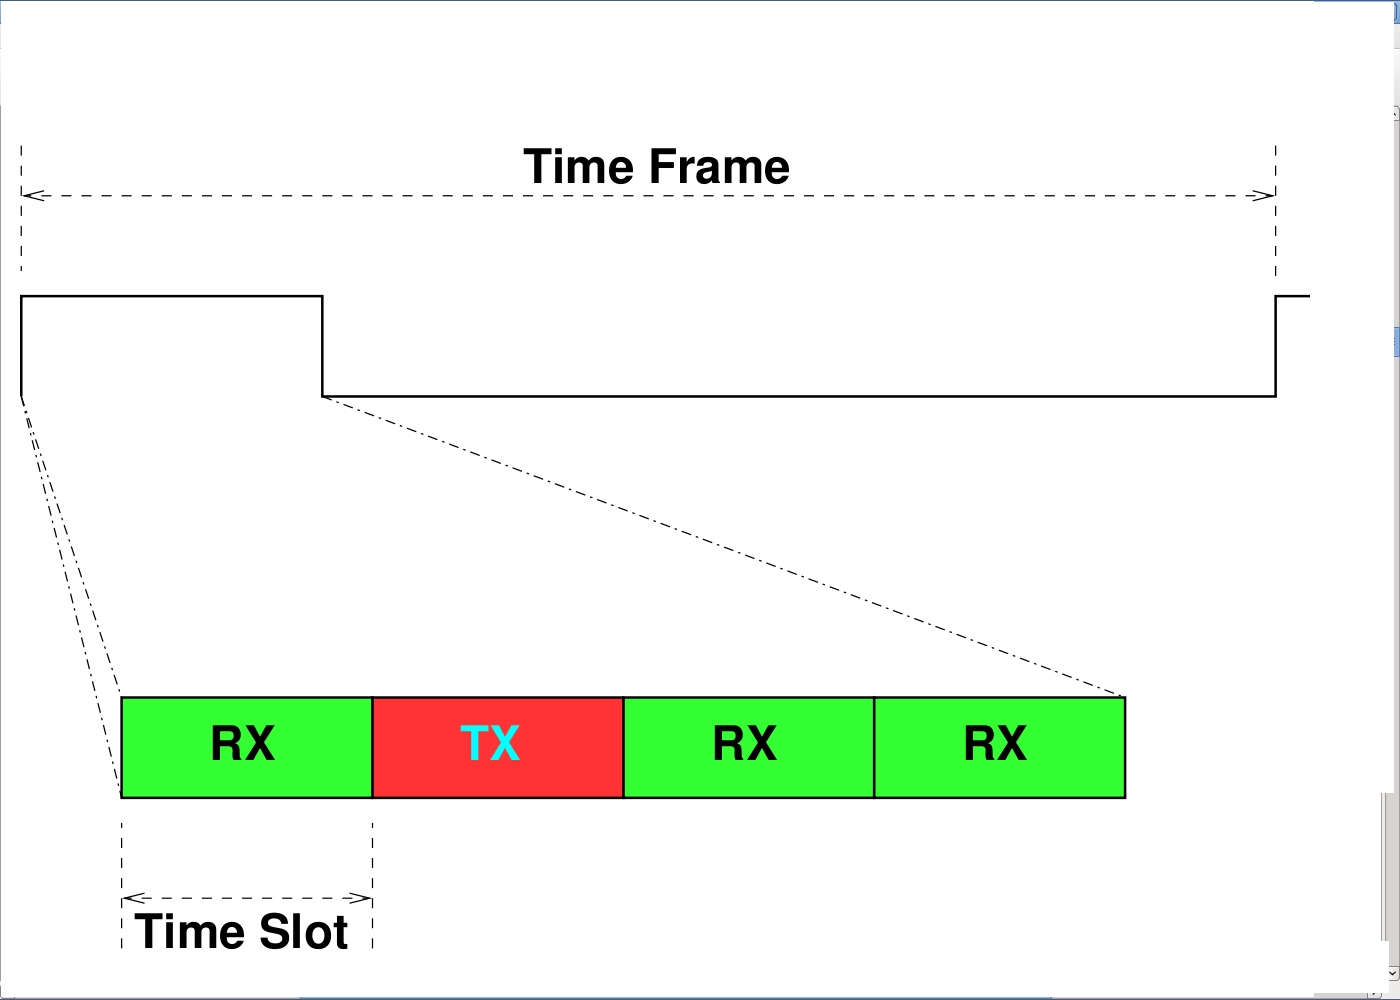
\includegraphics[width=0.8 \textwidth]{tdma_slot}
 \caption{TDMA Slot}
\end{figure}
\end{frame}


\begin{frame}
\begin{figure}
 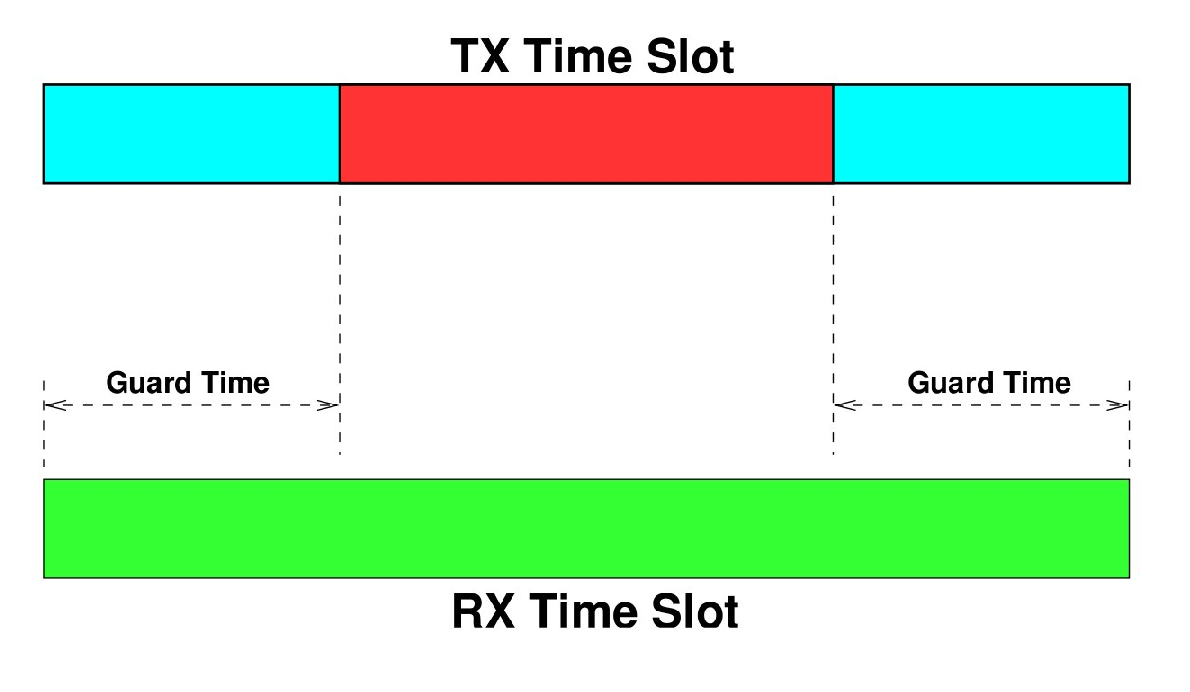
\includegraphics[width=0.8\textwidth]{a_slot}
 \caption{TDMA guard time}
\end{figure}
\end{frame}

\begin{frame}
    \frametitle{Frequency of Synchronization}
\textit{Worst case scenario - Clocks drifting in opposite
directions}
\begin{equation}
t_{guard} = f_{sy}[\Delta f_{sl} + \Delta f_{fa}]
\end{equation}
$where$
\begin{equation}
 t_{guard} = 274.6575 \mu s
\end{equation}
\newline
\textit{The maximum value will be}
\begin{center}
$f_{sy}= 4 $\end{center}
\end{frame}

\begin{frame}
    \frametitle{Node Time}
    \begin{figure}
     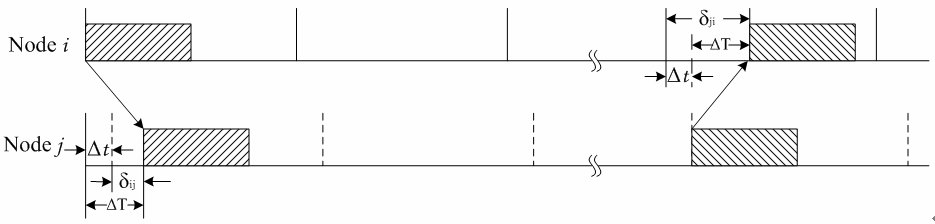
\includegraphics[width=0.8 \textwidth]{node_time}
    \end{figure}
        $\Delta T$ \textit{is the time difference between the nodes firing
        times}
    \newline
    $\Delta t$ \textit{is the delay(transmitting , receiving and propagation
    delay)} \newline
    $\delta_{ij}$ \textit{is the net difference in time}
\end{frame}
\begin{frame}
    \frametitle{Adjusting the error}
    \begin{equation}
         \tilde t_{i} = I_i + \frac{f_i(t)}{f_o}t + D_i  ,
    \end{equation}
    \newline
    \textit{
where \newline
 $I_i$ is the initial firing time of the node ,\newline
 $f_i$ is the frequency of the node at time t ,\newline
 $f_o$ is the nominal frequency of the node's clock , \newline
 $D_i$ is the processing time(Upon receiving and transmitting) plus the delay in propagation}
\end{frame}

\begin{frame}
    \frametitle{Adjusting the error}
\begin{equation}
\Delta t_{ij} = \tilde t_i  - \tilde t_j  ,
\end{equation}
\newline
\begin{equation}
 \Delta t_{ij} = (I_i - I_j) + (D_i-D_j) + t(f_i - f_j) ,
\end{equation}
\newline
\begin{equation}
\tilde{t_i} = t_i + O_i ,
\end{equation}
\newline
where $O_i$ is given by \newline
\begin{equation}
O_i = f(\Delta t_{ij}) ,
\end{equation}
\end{frame}
\begin{frame}
\begin{figure}[ht]
\includemovie[
  poster,
  text={\small(Loading Circle-m-increase3.mp4)}
]{6cm}{6cm}{movie.mpeg}
\end{figure}
\end{frame}
\begin{frame}
 \frametitle{Gradient Clock Synchronization}
  Assumption: Perfect Clock - No drift \newline \newline
  The tightest possible worstcase synchronization between two nodes which are $d$ apart is
  \begin{equation}
   \Omega(d)
  \end{equation}
  where \newline
  $d$ is the delay between the receiver and the sender nodes,\newline
  \newline
\end{frame}
\begin{frame}
 \frametitle{Gradient Clock Synchronization}
  Assumption: Perfect Clock - No drift \newline \newline
  But the lower bound of the skew between the clocks when the network grows beyond two nodes is
  \begin{equation}
   \Omega(d + \frac{logD}{loglogD})
  \end{equation}
\newline
  where \newline \newline
  $D$ is the maximum delay between two nodes in the network. \newline
  \newline
  Even if the maximum delay between two nodes remains constant, the lower bound increases as the network grows.
\end{frame}

\section{Intermediate Results}

\begin{frame}
\frametitle{Algorithm} Mean \newline
\begin{equation}
O_i = Mean(\Delta t_{ij})
\end{equation}
Median \newline
\begin{equation}
O_i = Mean(\Delta t_{ij})
\end{equation}
Least Square Curve fitting \newline
\begin{equation}
O_i = f(\Delta t_{ij}) ,
\end{equation}
where $f(x)$ is a curve fitting function.
\end{frame}
\begin{frame}
    \frametitle{Output}
    \begin{figure}
    \centering
    \includegraphics[width=0.75 \textwidth]{output}
    \caption{Synchronization error for Moving Nodes- speed in Km/hr}
    \end{figure}
\end{frame}

\begin{frame}
    \frametitle{Output}
    \begin{figure}
    \centering
    \includegraphics[width=0.75 \textwidth]{output}
    \caption{Synchronization error for Moving Nodes- speed in Km/hr}
    \end{figure}
\end{frame}

%\begin{frame}
%   \frametitle{Output}
%    \begin{figure}
%    \centering
%    \includegraphics[width=0.75 \textwidth]{output}
%    \caption{Synchronization error for Moving Nodes -$10 Km/hr$}
%    \end{figure}
%\end{frame}

\begin{frame}
    \frametitle{Output}
    \begin{figure}
    \centering
    \includegraphics[width=0.75 \textwidth]{output}
    \caption{Effect of the gain factor- Static Nodes with interferance}
    \end{figure}
\end{frame}

\section{Discussion Points}

\begin{frame}
    \frametitle{Discussion Points}
    \begin{itemize}
    \item Generic algorithm development \newline
    \item Calculations on how can the slot allocation algorithm cope without synchornization \newline
    \item Computational complexity, fast convergence, stability \newline
    \item Gurad time tradeoff \newline
    \item Application Sensitivity ????  \newline
    \item Simulation Environment \newline
    \item Size of the Network and the bound on Synchronization limit
    \end{itemize}
\end{frame}
\end{document}